\documentclass[conference]{IEEEtran}

\usepackage{amsmath, amsthm, amssymb, dsfont, accents}

\usepackage{tikz}
\usepackage{hyperref, booktabs}
\usepackage{biblatex}

\usetikzlibrary{calc, automata}

\addbibresource{2_references.bib}

\pdfinfo{
   /Author (Homer Simpson)
   /Title  (Robots: Our new overlords)
   /CreationDate (D:20101201120000)
   /Subject (Robots)
   /Keywords (Robots;Overlords)
}

% MDPs
\newcommand{\MDP}{\mathbb{M}}

\newcommand{\X}{\mathbb{X}}
\newcommand{\U}{\mathbb{U}}
\newcommand{\init}{\rho}
\newcommand{\tr}{T}

\newcommand{\pol}{\mu}

% LTL
\newcommand{\True}{\texttt{true}}
\newcommand{\False}{\texttt{false}}
\newcommand{\AP}{AP}

\newcommand{\ltluntil}{\mathcal{U}}
\newcommand{\ltlnext}{\bigcirc}

\newcommand{\alphabet}{{2^{\AP}}}
\newcommand{\word}{\boldsymbol{\pi}}
\newcommand{\letter}{\pi}
\newcommand{\lab}{L}

\newcommand{\FSA}{\mathcal{A}}

% Probability
\newcommand{\Prob}{\mathbf{P}}


% Value iteration
\newcommand{\bellman}{\mathcal{B}}


% Math
\DeclareMathOperator*{\argmin}{arg\,min}
\DeclareMathOperator*{\argmax}{arg\,max}
\newcommand{\ind}{\mathbf{1}}


\newtheorem{problem}{Problem}
\newtheorem{definition}{Definition}
\newtheorem{remark}{Remark}
\newtheorem{example}{Example}

\newcommand{\red}[1]{{\color{red} #1 }}

\begin{document}

\title{\huge Sequential Value Iteration for Modular Systems Applied to Collaborative Space Robotics}

\author{PN et al}

\maketitle

\begin{abstract}
  As a step towards achieving autonomy in space exploration missions, we consider a collaborative robotic system with a copter and a rover. The copter explores an unknown environment so as to maximize the probability that the rover can satisfy a science mission expressed in Linear Temporal Logic. We mitigate the curse of dimensionality for this large system by leveraging its decomposed nature, and by using sparse tensor product representations for value function and control policy. With hardware experiments we demonstrate that the resulting policy makes intelligent decisions in the face of uncertainty.
\end{abstract}

\IEEEpeerreviewmaketitle

	
%%%%%%%%%%%%%%%%%%%%%%%%%%%%%%%%%%%%%%%%%%%%%%%%
%%%%%%%%%%%%%%%%%%%%%%%%%%%%%%%%%%%%%%%%%%%%%%%%

\section{Introduction}

\begin{itemize}
  \item Main (potential) contributions:
  \begin{itemize}
    \item Reactive control in environment belief space
    \item Contract with low-level safety-critical? controller
    \item Cooperative robotics (copter explores to maximize probability that rover can satisfy spec)
    \item Efficient sequential value iteration for product MDPs
    \item More difficult: label-based abstraction for quadrotor (belief or non-belief) dynamics?? 
  \end{itemize}
\end{itemize}

\begin{itemize}
  \item Work for literature review
  \begin{itemize}
    \item \cite{Papusha2016}
    \item \cite{Alora2016}
    \item Maybe (need to read): \cite{Lavaei2017}
  \end{itemize}
\end{itemize}

\subsection{Preliminaries}

\begin{itemize}
  \item $\mathcal P(\X)$: probability densities over $\X$
\end{itemize}

\subsection{Paper layout}

\section{Markov Decision Processes and Temporal Logics}

We give definitions related to Markov Decision Process (MDPs), followed by basic concepts related to linear temporal logics.

\subsection{Markov Decision Processes}

We first define Markov decision processes over finite state spaces as follows \cite{hll1996}.
% \cite{mt1993,bertsekas2004stochastic}.
\begin{definition}
\label{def:MDP}
  A discrete-time \textbf{Markov decision process} (MDP) is a tuple $\MDP = (\X, \init, \tr, \U)$ where
  \begin{itemize}
    \item $\X$ is a (finite) state space with states $x\in\X$; % as its elements;
    \item $\init \in \mathcal P(\X)$ is an initial probability distribution;
    \item $\U$ is a (finite) input space with inputs $u\in\U$;
    \item $\tr$ is a conditional stochastic kernel that assigns to each state $x\in \X$ and control $u\in \U$ a probability density $\tr(\cdot\mid x,u)$ over $\X$.
  \end{itemize}
\end{definition}

An execution of $\MDP$ is a state-input sequence $(x_0, u_0)(x_1, u_1)\ldots$ where $x_0 \sim \rho$ and $x_{k+1} \sim \tr(\cdot \mid x_k, u_k)$ for inputs $u_k \in \U$. 

\subsection{Specifications}

\begin{itemize}
  \item Something about atomic propositions (and examples)
\end{itemize}

Consider a set $AP = \{ p_1, \ldots, p_L \}$ of atomic propositions; it defines an \emph{alphabet} $\alphabet$ where each \emph{letter} $\letter$ of the alphabet is defined as a set of atomic propositions. An infinite string of letters is a \emph{word} $\word=\letter_0\letter_1\letter_2\ldots\in\alphabet^{\mathbb{N}}$.

To quantify the dynamic behavior of a system, we define the word associated to an MDP execution. Consider a labeling function $\lab: \X \rightarrow \alphabet$ that maps states to letters in the alphabet. The words generated by a belief trajectory $\mathbf{x} = x_0 x_1 x_2 \ldots$ can be defined as the word $\word = \lab(x_0)\lab(x_1) \lab(x_2) \ldots$. System properties can now be expressed via temporal logic formulas over the generated words.

Properties are formulas composed of atomic propositions and operators. In the sequel we focus on a fragment of linear temporal logic. 
\begin{definition}
  \label{def:gdtl-syntax}
  Formulas in the \textbf{syntactically co-safe LTL} (scLTL) fragment are constructed according to the grammar
  \begin{equation*}
    \label{eq:scLTL}
    \psi =  \True \ |\ p \ |\ \lnot p \ |\ \psi_1 \vee\psi_2  \ |\ \psi_1 \land \psi_2 \ |\ \psi_1 \ltluntil \psi_2 \ |\ \ltlnext \psi,
  \end{equation*}
  where $p\in \AP$ is an atomic proposition.
\end{definition}

% The syntax defines the symbols and their correct ordering to form a formulae.
To define the interpretation of a formula, i.e. the \emph{semantics}, consider a word $\word$.

\begin{definition}
 The \textbf{semantics} of scLTL are defined recursively as follows: $\word$ \textbf{satisfies} $\psi$ at time $k$, written $(\word, k) \models \psi$, if
 \begin{itemize}
    \item $(\word, k) \models \True$;
    \item $(\word, k) \models p$ iff $p \in \letter_k$;
    \item $(\word, k) \models \psi_1 \land  \psi_2  $ iff $ ( (\word, k) \models \psi_1 ) \land ( (\word, k) \models \psi_2 ) $;
    \item $(\word, k) \models \psi_1 \lor  \psi_2  $ iff $ ( (\word, k) \models \psi_1 ) \lor ( (\word, k) \models \psi_2 ) $;
    \item $(\word, k) \models  \psi_1 \ltluntil \psi_2 $ iff $\exists j \geq k \text{ s.t. } ((\word, j) \models \psi_2 ) $ and $(\word, l) \models \psi_1, \forall l \in \{k, \ldots j-1\}$;
    \item $(\word, k) \models \ltlnext \psi$ iff $(\word, k+1) \models \psi$.
 \end{itemize}

\end{definition}

We say that a trajectory $\mathbf{x} = x_0 x_1 x_2 \ldots$ satisfies a specification $\psi$, written $\mathbf{x} \models \psi$, if the generated word $\word =\lab(x_0) \lab(x_1) \lab(x_2) \ldots$ satisfies $\psi$ at time 0, i.e. $\word_0 \models \psi$.

\subsection{Problem Statement}

The objective of this work is to design a policy $\pol$ such that a specification $\psi$ is satisfied with a given probability.
\begin{problem}
\label{prob:main}
  Consider a model $\MDP = (\X, \rho, \tr, \U)$ generating trajectories $\mathbf{b} = x_0 x_1 x_2 \ldots$, a labeling function $\lab : \X \rightarrow AP$, and a scLTL formula $\psi$ defined over $AP$. Construct a policy $\pol$ such that
  \begin{equation}\label{eq:probstatement}
    \Prob_\init^\pol ( \mathbf{b} \models \psi )\geq p,
  \end{equation}
  where $p$ is either given or to be maximized.
\end{problem}

\subsection{Policy Synthesis via Value Iteration}

Policy synthesis for a scLTL specification over a space $\X$ is equivalent to reachability of $\X\times Q_f$ on the product system $\MDP \otimes \FSA_\psi$. In this case, the Bellman operator is
\begin{equation}
\label{eq:V_recopt_inf_mu}
%\begin{aligned}
  \bellman_\pol (\mathbf V)(b,q)\! = \hspace{-1mm} \int_{\X} \hspace{-1mm} \max \left( \mathbf 1_{Q_f}(q'), \!\mathbf V( b'\!, q') \right)\! {\tr}(\mathrm{d} b' |b,\pol(b,q))\!
%\end{aligned}
\end{equation}
with the implicit DFSA transitions  $q' =\delta_\FSA(q,\lab(b'))$, %\red{$\mathrm{d} b'= d b'\times\{q'\}$},
and similarly for the policy-optimal version $\bellman_*$.  For the converged value function $\mathbf V^\infty_* =  \lim_{K\rightarrow\infty}\bellman_*^K\! \mathbf V^0$, now expresses the value of
\begin{equation}
\label{eq:prob:_optimal} 
 \sup_{\pol}\mathbf{P}_\init^{\pol}( {\mathbf{b}} \vDash\! \psi)\! =\!
  \int_{\X} \! \max \left( \mathbf 1_{Q_f}( q'), 
   \mathbf V^\infty_*(x_0, q') \right) \init(\mathrm{d} x_0) \!
\end{equation}
with the associated deterministic and stationary policy $ \pol_*=(\pol_*,\pol_*,\ldots)$ obtained as the maximizing argument. 
This policy defined for the product MDP $\MDP \otimes \FSA_\psi$, maps to control actions as a function of the state $(b,q) \in \X \times Q$, and can be translated to a non-stationary policy for the original MDP $\MDP$ that includes $\FSA_\psi$ as a memory model.


\section{Sequential Value Iteration}


\subsection{Networks of MDPs}

Consider two MDPs $\MDP_1 = (\X_1, \init_1, \U_1, \tr_1)$ and $\MDP_2 = (\X_2, \init_2, \U_2, \tr_2)$. Next we introduce the parallel and serial products between the two.
\begin{definition}
  The \textbf{parallel product} of $\MDP_1$ and $\MDP_2$ is the MDP 
  \begin{equation}
    \MDP_1 \otimes_{par} \MDP_2 = (\X_1 \times \X_2, \init_{par}, \U_1 \times \U_2, \tr_{par}),
  \end{equation}
  where
  \begin{equation}
    \init_{par}(x_1, x_2) = \init_1(x_1) \init_2(x_2)
  \end{equation}
  and
  \begin{equation}
  \begin{aligned}
      \tr_{par}&(x_1', x_2' \mid x_1, x_2, u_1, u_2) \\
      & = \tr_1 (x_1' \mid x_1, u_1) \tr_2 (x_2' \mid x_2, u_2)
  \end{aligned}
  \end{equation}
\end{definition}

\begin{definition}
  The \textbf{serial product} of $\MDP_1$ and $\MDP_2$ given a \textbf{connection} $C : \X_1 \rightarrow \U_2$ is the MDP 
  \begin{equation}
    \MDP_1 \otimes_{ser} \MDP_2 = (\X_1 \times \X_2, \init_{ser}, \U_1, \tr_{ser}),
  \end{equation}
  where
  \begin{equation}
    \init_{ser}(x_1, x_2) = \init_1(x_1) \init_2(x_2)
  \end{equation}
  and
  \begin{equation}
  \begin{aligned}
      \tr_{ser}&(x_1', x_2' \mid x_1, x_2, u_1) \\
      & = \tr_1 (x_1' \mid x_1, u_1) \tr_2 (x_2' \mid x_2, C(x_1') )
  \end{aligned}
  \end{equation}
\end{definition}
That is, a transition $x_1 \rightarrow x_1'$ in $\MDP_1$ triggers an action $C(x_1')$ in $\MDP_2$ that results in a transition in $x_2' \sim T_2(\cdot \mid x_2, C(x_1'))$

\begin{itemize}
  \item \red{Can we do more general MDP graph?}
\end{itemize}

\subsection{Sequential Iteration of Bellman Operator}

\begin{itemize}
  \item \red{Can we include action in Bellman op?}
\end{itemize}

Given a function $g: \X \times \mathbb{R}_+ \rightarrow \mathbb{R}_+$, consider a general Bellman operator $\bellman : (\X \rightarrow \mathbb{R}_+) \rightarrow (\X \rightarrow \mathbb{R}_+)$ on the following form:
\begin{equation}
  (\bellman V) (x) = \max_{\pol \in (\X \rightarrow \U)} \sum_{x' \in \X}  g(x', V(x')) T(x' \mid x, \pol(x)).
\end{equation}
The optimal value function $V^*$ and policy $\pol^*$ for a given bellman operator $\bellman$ is found via the iterations
\begin{subequations}
  \begin{align}
    & V^*_0 \equiv 0, \\
    & V^*_{k+1}  = \bellman V_k \label{eq:iter}, \\
    & \pol^* \in \argmax_{\pol \in (\X \rightarrow \U)} \sum_{x' \in \X}  g(x', V^*(x')) T(x' \mid x, \pol(x)).
  \end{align}
\end{subequations}

\begin{example}
  For the Bellman operator corresponding to reaching a set $X_f$, the function $g$ is given by
  \begin{equation*}
    g(x', v') = \max( \ind_{X_f}(x'), v').
  \end{equation*}
\end{example}

\begin{example}
  Consider the finite-horizon optimal control problem 
  \begin{equation}
     \max \sum_{t=0}^T J_t(x_t).
  \end{equation} 
  In this case, if the dynamics programming is initialized with $V_T(x) = J_T(x)$, iterated applications of the Bellman operator corresponding to $g_t(x', v') = J_{t-1}(x') + v'$, i.e.
  \begin{equation*}
    V_{t-1}(x) = \bellman_t V_{t} (x) = \max_{\pol} (J_{t-1}(x') + V_{t}(x')) T(x' \mid x, \pol(x))
  \end{equation*}
  computes the value function at times $T-1, T-2, \ldots, 0$.
\end{example}

We now consider the Bellman iteration step for parallel and serial product MDPs. For a parallel MDP we get
\begin{equation*}
\begin{aligned}
  \max_{\pol: (\X_1 \times \X_2 \rightarrow \U_1 \times \U_2)} \sum_{x_1', x_2' \in \X_1 \times \X_2}  g(x_1', x_2', V^*(x_1', x_2')) \\
  \times T_{par}(x_1', x_2' \mid x_1, x_2, \pol(x_1, x_2)) \\
  = \max_{\pol: (\X_1 \times \X_2 \rightarrow \U_1 \times \U_2)} \sum_{x_1' \in \X_1} T_1(x_1' \mid x_1, \pol(x_1, x_2)) \\
    \sum_{x_2' \in \X_2}  g(x_1', x_2', V(x_1', x_2')) T_2(x_2' \mid x_2, \pol(x_1, x_2)).
\end{aligned}
\end{equation*}
It follows that the Bellman update $V \mapsto \bellman V$ for a parallel product can be computed sequentially as follows:
\begin{equation}
\begin{aligned}
  W_2(x_1', x_2') &= g(x_1', x_2', V(x_1', x_2')) \\
  W_1(x_1, x_1', x_2) &= \max_{\pol_2: \X_1 \times \X_2 \rightarrow \U_2} \sum_{x_2' \in \X_2}  T_2(x_2' \mid x_2, \pol_2(x_1, x_2)) W_2(x_1', x_2')  \\
  \bellman V(x_1, x_2) &= \max_{\pol_1: \X_1 \times \X_2 \rightarrow \U_1}  \sum_{x_1' \in \X_1}  T_1(x_1' \mid x_1, \pol_1(x_1, x_2)) W_1(x_1', x_2)
\end{aligned}
\end{equation}

\red{
\begin{itemize}
  \item Decomposition requires that $W_1$ is independent of $x_1$. Satisfied if:
  \begin{itemize}
    \item Decentralized policy is optimal. When is this true?
    \item We consider policy $\mu_2 = \mu_2(x_1', x_2)$ (i.e. $\MDP_1$ moves first).
    \item If there is no policy maximization (e.g., if it is part of a serial product)
  \end{itemize}
\end{itemize}

}

For a serial product we get
\begin{equation*}
\begin{aligned}
  \bellman V (x_1, x_2) & = \max_{\pol: (\X_1 \times \X_2 \rightarrow \U_1)} \sum_{x_1', x_2' \in \X_1 \times \X_2}  g(x_1', x_2', V(x_1', x_2')) \\
  & \quad \times T_{ser}(x_1', x_2' \mid x_1, x_2, \pol(x_1, x_2)) \\
  & = \max_{\pol: (\X_1 \times \X_2 \rightarrow \U_1)} \sum_{x_1' \in \X_1} T_1(x_1' \mid x_1, \pol(x_1, x_2)) \\
  & \quad \times \sum_{x_2' \in \X_2}  g(x_1', x_2', V(x_1', x_2')) T_2(x_2' \mid x_2, C(x_1')).
\end{aligned}
\end{equation*}
It follows that the Bellman update $V \mapsto \bellman V$ for a serial product can be computed sequentially as follows:
\begin{equation*}
\begin{aligned}
  W_2(x_1', x_2') & = g(x_1', x_2', V(x_1', x_2')) \\
  W_1(x_1', x_2) & = \sum_{x_2' \in \X_2}  T_2(x_2' \mid x_2, C(x_1')) W_2(x_1', x_2'), \\
  \bellman V(x_1, x_2) & = \max_{\pol: (\X_1 \times \X_2 \rightarrow \U_1)} \sum_{x_1' \in \X_1} T_1(x_1' \mid x_1, \pol(x_1, x_2)) W_1(x_1', x_2).
\end{aligned}
\end{equation*}
As a consequence, the Bellman recursion can be computed without computing the transition matrices for the aggregate system $\MDP_1 \otimes_{ser} \MDP_2$. That is, instead of dealing with objects of size $\mathcal O(| \X_1 \times \X_2 |^2)$, we can deal with objects of size $\mathcal O(|\X_1|^2 + |\X_2|^2)$. The procedure generalizes to serial products of arbitrary length with a potential for significant computational savings. 

\red{Is this well known/trivial??}

\begin{example}
  \red{TODO: Run some randomized experiments (with dense and sparse matrices) to show how sequential value iteration performs against centralized value iteration.}
\end{example}

\begin{remark}
  In serial products of arbitrary length a connection $C_i$ can be defined either as $C_i: \X_{i-1} \rightarrow \U_i$, or as $C_i: \X_1 \times \ldots \times \X_{i-1} \rightarrow \U_i$. In the latter case the connection potentially becomes a non-sparse object. \red{Can we restrict the format of the connection to allow for a sparse representation?}
\end{remark}

\begin{remark}
  \red{Talk about extension to non-deterministic products by introducing a minimization term. Point out connection to errors in abstractions.} 
\end{remark}

\subsection{Sparse Value Function via Tensor Products}

In the previous subsection we outlined how Bellman iterations for a value function can be performed sequentially in product systems. However, a dense value function representation is still of size $\mathcal O (|\X_1| |\X_2|)$ which can constitute a bottleneck for large products. In this section we explore how computational efficiency can be improved by using sparse value function representations. The cost is a loss of precision and guarantees in the final value function.

\begin{itemize}
  \item \red{No theory for this section yet, don't know if its possible...}
\end{itemize}

\section{Case Study}

\red{Variations of problems to solve (decreasing order of difficulty/desirability):
\begin{itemize}
  \item Simultaneous rover/copter execution
  \item Copter maps in a way that maximizes success probability of rover (1. copter execution, 2. rover execution)
  \item Exclude rover and consider specification related to copter only
\end{itemize}}

\begin{figure}
  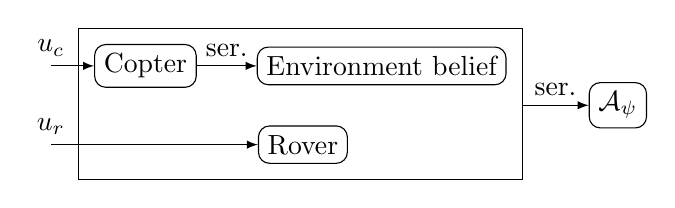
\begin{tikzpicture}
    \node[draw, node distance=3cm, rounded corners] (copter) {Copter};
    \node[draw, node distance=3cm, rounded corners, right of=copter] (environment) {Environment belief};
    \node[xshift=-1cm, draw, node distance=1cm, rounded corners, below of=environment] (rover) {Rover};
    \node[yshift=-0.5cm, draw, node distance=3cm, rounded corners, right of=environment] (fsa) {$\FSA_\psi$};

    \draw ([xshift=-2mm, yshift=2mm]$(copter.north west)$) rectangle ([xshift=2mm, yshift=-2mm]$ (rover.south west)!(environment.east)!(rover.south east) $) node[coordinate] (east) {};

    \draw[-latex] (copter) -- node[above] {ser.} (environment);
    \draw[latex-] (fsa) -- node[above] {ser.} ($(fsa.west)!(east)!($(fsa.west)-(1,0)$)$);

    \draw[latex-] (copter) -- ++(-1.2,0) node[coordinate] (west) {} node[above] {$u_c$};
    \draw[latex-] (rover) -- ($(rover.west)!(west)!(rover.east)$) node[above] {$u_r$};
  \end{tikzpicture}
  \caption{Illustration of aggregate system constructed as parallel and serial products.}
  \label{fig:agg}
\end{figure}

We consider three system components $\MDP_{copt}$, $\MDP_{rov}$, and $\MDP_{env}$, representing abstract dynamics of the copter and rover, and environment belief state dynamics. Adding a specification automaton, the aggregate system is the product system illustrated in Figure \ref{fig:agg}:
\begin{equation}
  ((\MDP_{copt} \otimes_{ser} \MDP_{env}) \otimes_{par} \MDP_{rov}) \otimes_{ser} \FSA_\psi
\end{equation}
That is, the Copter provides input to the map in a serial product, and the combined system provides input to a specification DFSA $\FSA_\psi$. 

\paragraph{Abstract Robot Models:}

For now, $n \times n$ grid with free movement. Copter also has a clock $\MDP_{clock}$ that limits total movement.

\paragraph{Low-level Robot Controllers:}

How quadrotors are controlled to move between grid cells. \red{Can we provide some guarantees under reasonable assumptions?}

\paragraph{Environment Belief Model:}

\begin{figure}
  \begin{center}
  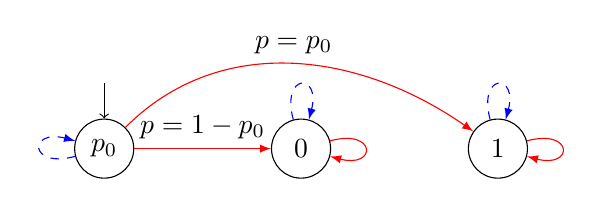
\begin{tikzpicture}
    \node[draw, minimum width=0.75cm, node distance=2.5cm, circle, initial above,initial text={} ] (b0) {$p_0$};
    \node[draw, minimum width=0.75cm, node distance=2.5cm, circle, right of=b0] (b1) {0};
    \node[draw, minimum width=0.75cm, node distance=2.5cm, circle, right of=b1] (b2) {1};

    \draw[-latex, red] (b0) to node[black, above] {$p = 1-p_0$} (b1);
    \draw[-latex, red] (b0) to[out=45, in=145] node[black, above] {$p = p_0$} (b2);

    \draw[-latex, blue, dashed] (b0) to[loop left] (b0);
    \draw[-latex, red] (b1) to[loop right] (b1);
    \draw[-latex, red] (b2) to[loop right] (b2);
    \draw[-latex, blue, dashed] (b1) to[loop above] (b1);
    \draw[-latex, blue, dashed] (b2) to[loop above] (b2);
  \end{tikzpicture}
  \end{center}
  \caption{Illustration of environment belief model for a single region. At the beginning the belief is $p_0$. When a measurement is received (solid red edges), the belief transitions to $1$ with probability $p_0$ and to $0$ with probability $1-p_0$. That is, one measurement is sufficient to determine the state of the region. When no measurement is taken (blue dashed edges), or if a measurement has already been taken, the state does not change.}
  \label{fig:envmdp}
\end{figure}

We assume that there are collections of regions of interest, where samples and/or obstacles may be located. Associated to each region is a belief state that evolves according to an MDP representing belief dynamics. A measurement is taken when the copter flies over a region.

\red{Can do simple model in Figure \ref{fig:envmdp}, or more elaborate Bernoulli model (next section)}


\paragraph{Specification:}

\begin{itemize}
  \item Rover should collect a sample and avoid obstacles
  \item Copter should land in safe area before battery is exhausted
\end{itemize}

\section{Bernoulli belief}

\subsection{Belief model}

Suppose we want to estimate an unknown label $\bar l \in \{ 0,1 \}$.
\begin{itemize}
  \item Prior distribution: $p(\bar l) = \begin{cases}
    q   & \bar l=0 \\
    1-q & \bar l=1
  \end{cases}$
  \item Measurement $m \sim p(m \mid \bar l) = \begin{cases}
    s & \bar l=0, m = 0, \\
    1-s & \bar l=0, m=1, \\
    s & \bar l=1, m= 1, \\
    1-s & \bar l=1, m=0.
  \end{cases}$ with accuracy $s > 1/2$.
\end{itemize}
We can thus write the posterior as
\begin{equation}
  p(\bar l \mid m) \propto p(m \mid \bar l) p(\bar l) = \begin{cases}
    q s & \bar l=0, m=0, \\
    q(1-s) & \bar l=0, m=1, \\
    (1-q) s & \bar l=1, m=1, \\
    (1-q)(1-s) & \bar l=1, m=0.
  \end{cases}
\end{equation}
After re-normalizing we can the update $q$ depending on the measurement $m$ as 
\begin{equation}
  q \mapsto \begin{cases}
    \frac{qs}{qs + (1-q)(1-s)} & m = 0, \\
    \frac{q(1-s)}{q(1-s) + (1-q)s} & m = 1, 
  \end{cases}
\end{equation}
These are the dynamics of the belief state. We assume that $m$ is sampled from the current belief $p(\bar l)$ which results in an MDP with state $q$ and action $s$:
\begin{equation}
\label{eq:bernoulli_mdp}
\begin{aligned}
  q & \longrightarrow \frac{qs}{qs + (1-q)(1-s)} \quad &  \text{w.p} \; & qs + (1-q)(1-s) \\
  q & \longrightarrow \frac{q(1-s)}{q(1-s) + (1-q)s} \quad &  \text{w.p} \; & q(1-s) + (1-q)s 
\end{aligned}
\end{equation}

\subsection{Belief abstraction}

\subsubsection{Uniform abstraction}

Consider an abstract state $\tilde q$ such that $|q - \tilde q| \leq \epsilon$, in an abstraction with state discretization $\eta$. The abstract state $\tilde q$ is updated in synchrony with $q$ according to
\begin{equation}
\begin{aligned}
  \tilde q &  \longrightarrow \left \lfloor \frac{\tilde qs}{\tilde qs + (1-\tilde q)(1-s)} \right \rfloor_\eta \quad &  \text{if $q$ grows} \\
  \tilde q & \longrightarrow \left \lfloor \frac{\tilde q(1-s)}{\tilde q(1-s) + (1-\tilde q)s} \right \rfloor_\eta \quad &  \text{if $q$ shrinks}
\end{aligned}
\end{equation}
Let 
\begin{equation}
\begin{aligned}
  f_1(q,s) = \frac{qs}{qs + (1-q)(1-s)}, \\
  f_2(q,s) = \frac{q(1-s)}{q(1-s) + (1-q)s}.
\end{aligned}
\end{equation}
Then, 
\begin{equation*}
\begin{aligned}
  \mathbb{P} \left[ |q' - \tilde q'| \leq \epsilon \right] = \left[qs + (1-q)(1-s)\right] \\
  \times \mathds{1} \left[ |f_1(q,s) - f_1(\tilde q,s)| \leq \epsilon - \frac{\eta}{2} \right] \\ + \left[q(1-s) + (1-q)s \right] \times \mathds{1} \left[ |f_2(q,s) - f_2(\tilde q,s)| \leq \epsilon - \frac{\eta}{2} \right]
\end{aligned}
\end{equation*}
It can be shown that
\begin{equation*}
\begin{aligned}
  & |f_1(q,s) - f_1(\tilde q,s)| \\ 
  & \; = s(1-s) \frac{|q - \tilde q|}{(qs + (1-q)(1-s))(\tilde qs + (1-\tilde q)(1-s))}, \\
  & |f_2(q,s) - f_2(\tilde q,s)| \\ 
  & \; = s(1-s) \frac{|q - \tilde q|}{(q(1-s) + (1-q)s)(\tilde q(1-s) + (1-\tilde q)s)}.
\end{aligned}
\end{equation*}
Under the assumption $q = \tilde q$ it follows that
\begin{equation}
\begin{aligned}
  \mathbb{P} \left[ |q' - \tilde q'| \leq \epsilon \mid |q-\tilde q| \leq \epsilon \right] \geq 1 - \sqrt{\frac{s(1-s) \epsilon}{\epsilon - \frac{\eta}{2}}}.
\end{aligned}
\end{equation}

\begin{itemize}
  \item Pro: can use lowest $\bar s$ to get inequality that holds for all $s > \bar s$
  \item Con: relatively high $\delta$.
\end{itemize}

\subsubsection{Non-uniform abstraction}

For a fixed $s$, consider the sequence
\begin{equation}
  c_0 = 1/2, \; c_{k+1} = f_1(c_k, s).
\end{equation}
Let each interval $[c_k, c_{k+1}]$ represent an abstract state and construct corresponding abstract states partitioning $[0, 1/2]$. Then the abstract model will be bisimilar to \eqref{eq:bernoulli_mdp}. The reason is that 
\begin{equation}
  f_1(\cdot, s) \circ f_2(\cdot, s) = Id.
\end{equation}
To get a finite abstraction, the abstract states contained in $[0, \gamma]$ and $[1- \gamma, 1]$ can be lumped together.

\begin{itemize}
  \item Pro: exact abstraction for given $s$: $0$-simulation
  \item Con: is (probably) not $\delta$-simulation when there are multiple possible values of $s$
\end{itemize}

\paragraph{Commutative:} It holds that $f_1(\cdot, s) \circ f_1(\cdot, s') = f_1(\cdot, s') \circ f_1(\cdot, s)$ and similarly for $f_2$. Therefore the only thing affecting the estimate $q$ is the net number of positive measurements at each confidence level. For two confidence levels, we can then use the following abstract states:
\begin{equation}
  \{ (n_{s_1}, n_{s_2}) : n_{s_1}, n_{s_2} \in \mathbb{N} \}. 
\end{equation}
For a finite description, we can lump together states that yield values of $q$ very close to 1 or 0. We can get arbitrarily close to $\delta = 0$.

\section{Hardware Experiments}

\begin{itemize}
    \item Copter in CAST
\end{itemize}

\printbibliography

\end{document}

